\chapter{Introduction}


% % Some applications of marine (Underwater and Aerial drones), suvryeing and wind trubine inspection
% Marine robotics has emerged as a transformative technology across diverse domains requiring underwater operations. For example, the offshore energy sector increasingly relies on underwater and aerial robots for routine inspection of wind turbines, identifying structural damage that could compromise operational integrity. Similarly, the oil and gas industry utilizes specialized underwater vehicles for pipeline inspection, identifying potential leaks or structural weaknesses over vast underwater networks. Marine robotics also plays a pivotal role in environmental monitoring, archaeological surveying, and defense applications including mine countermeasures and underwater surveillance.


% % Need for autonomy
% Autonomous operation is crucuial, as it reduces human risk and also reliability of these technologies.


% % PRoblems with marine robotics and why itr needs advanced control


% Despite significant advances, marine robotics faces unique challenges to be deployed fully autonomously for operations. There is a need for high precision control algorithms to can handle highly non linear, high digrees of freedom system, while excuting complex menauvers and trajectories.
% b) Handling uncertainties in oepration conditions such as currents, winds and s on 

% b) Generic Control Algorithms that would apply to the diverse nature of different robots






\section{Marine Robotics: Advancing Autonomy for Underwater and Aerial Applications Through Optimal Control}

Marine robotics encompasses a diverse array of platforms, including remotely operated vehicles (ROVs), autonomous underwater vehicles (AUVs), unmanned surface vehicles (USVs), as well as unmanned aerial vehicles (UAVs) (see Fig. \ref{fig:underwater_robotics_applications}). These systems are increasingly vital across multiple domains. In the energy sector, they can perform essential inspections of offshore wind turbines and subsea pipelines, detecting critical structural defects or leaks. Beyond industry, applications span environmental monitoring, archaeological surveying, scientific research, and defense operations like mine countermeasures and surveillance.


\begin{figure*}[!h]
    \centering
    % First Row
    \begin{subfigure}[b]{0.44\textwidth}
        \centering
        \includegraphics[width=\textwidth]{Phd_thesis/figs/lark.png}
        \caption{Upteko inspection drone.}
        \label{fig:subfig1}
    \end{subfigure}
    \hfill
    \begin{subfigure}[b]{0.49\textwidth}
        \centering
        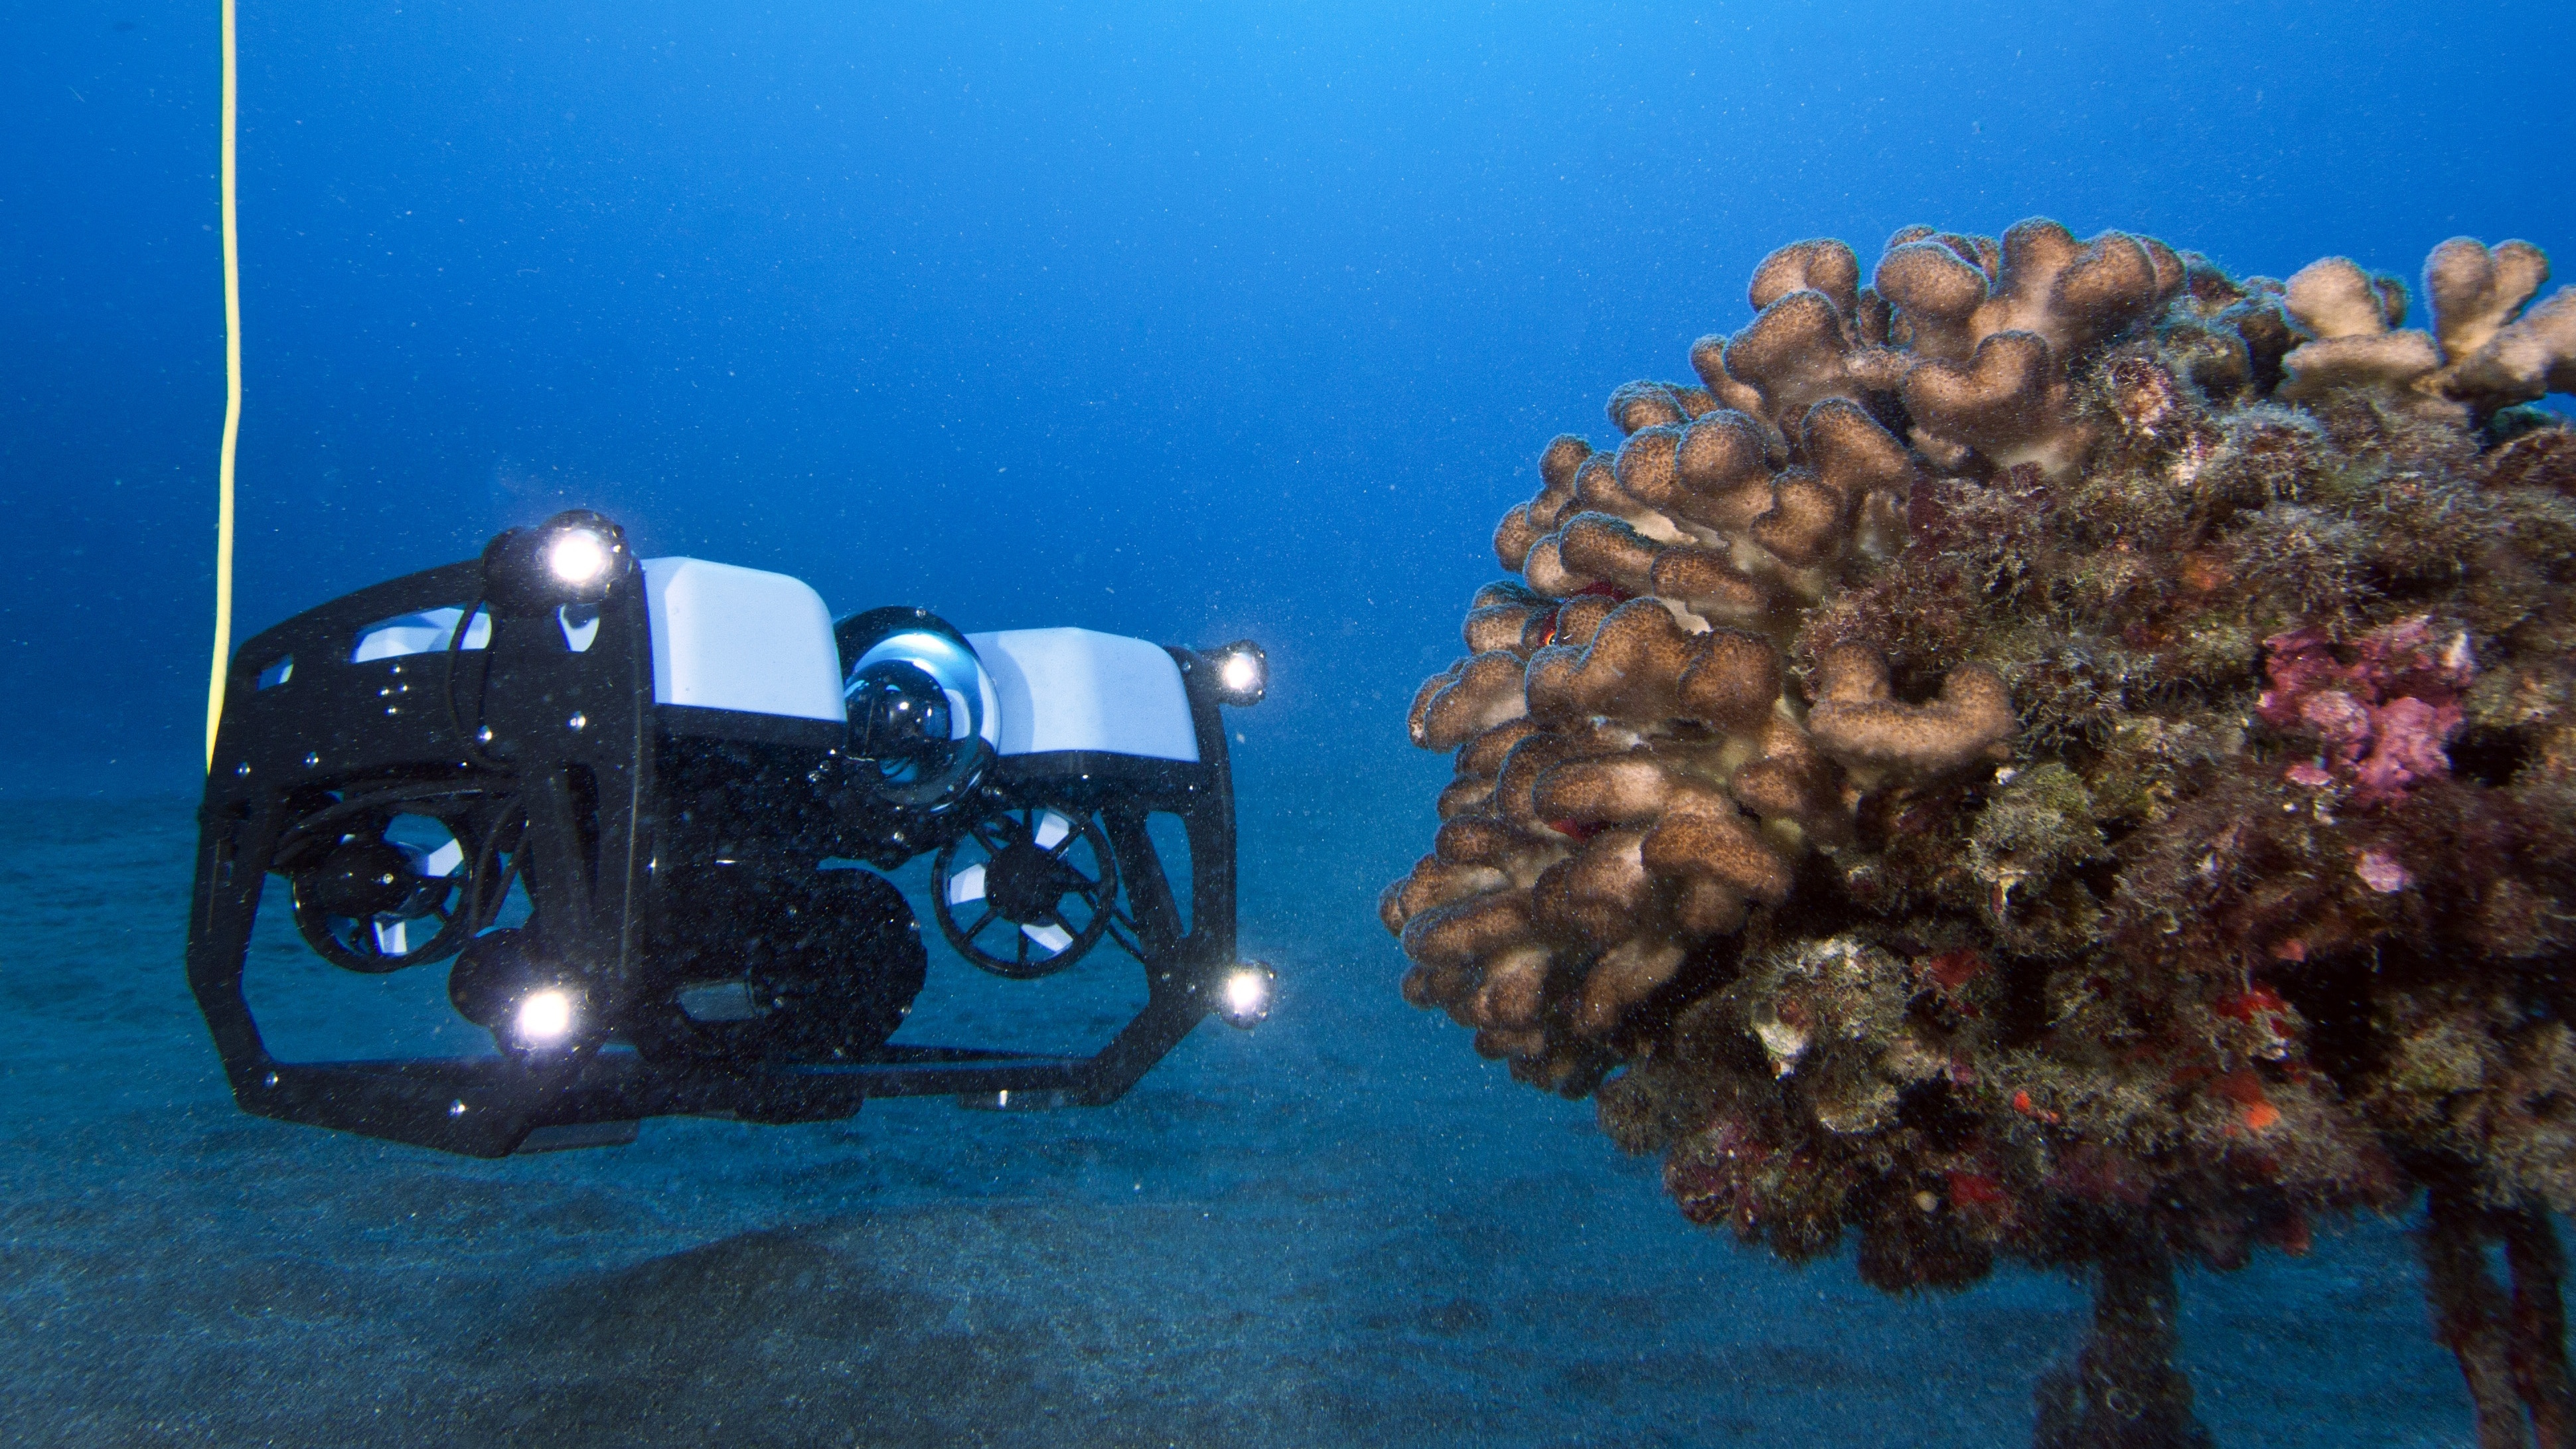
\includegraphics[width=\textwidth]{Phd_thesis/chapters/1.Introduction/figures/BlueROV2.jpg}
        \caption{BlueROV2 medium-sized tethered ROV \cite{bluerobotics_bluerov2_nodate}.}
        \label{fig:subfig2}
    \end{subfigure}
    
    \vspace{0.5cm} % Adjust vertical space between rows
    
    % Second Row
    \begin{subfigure}[b]{0.46\textwidth}
        \centering
        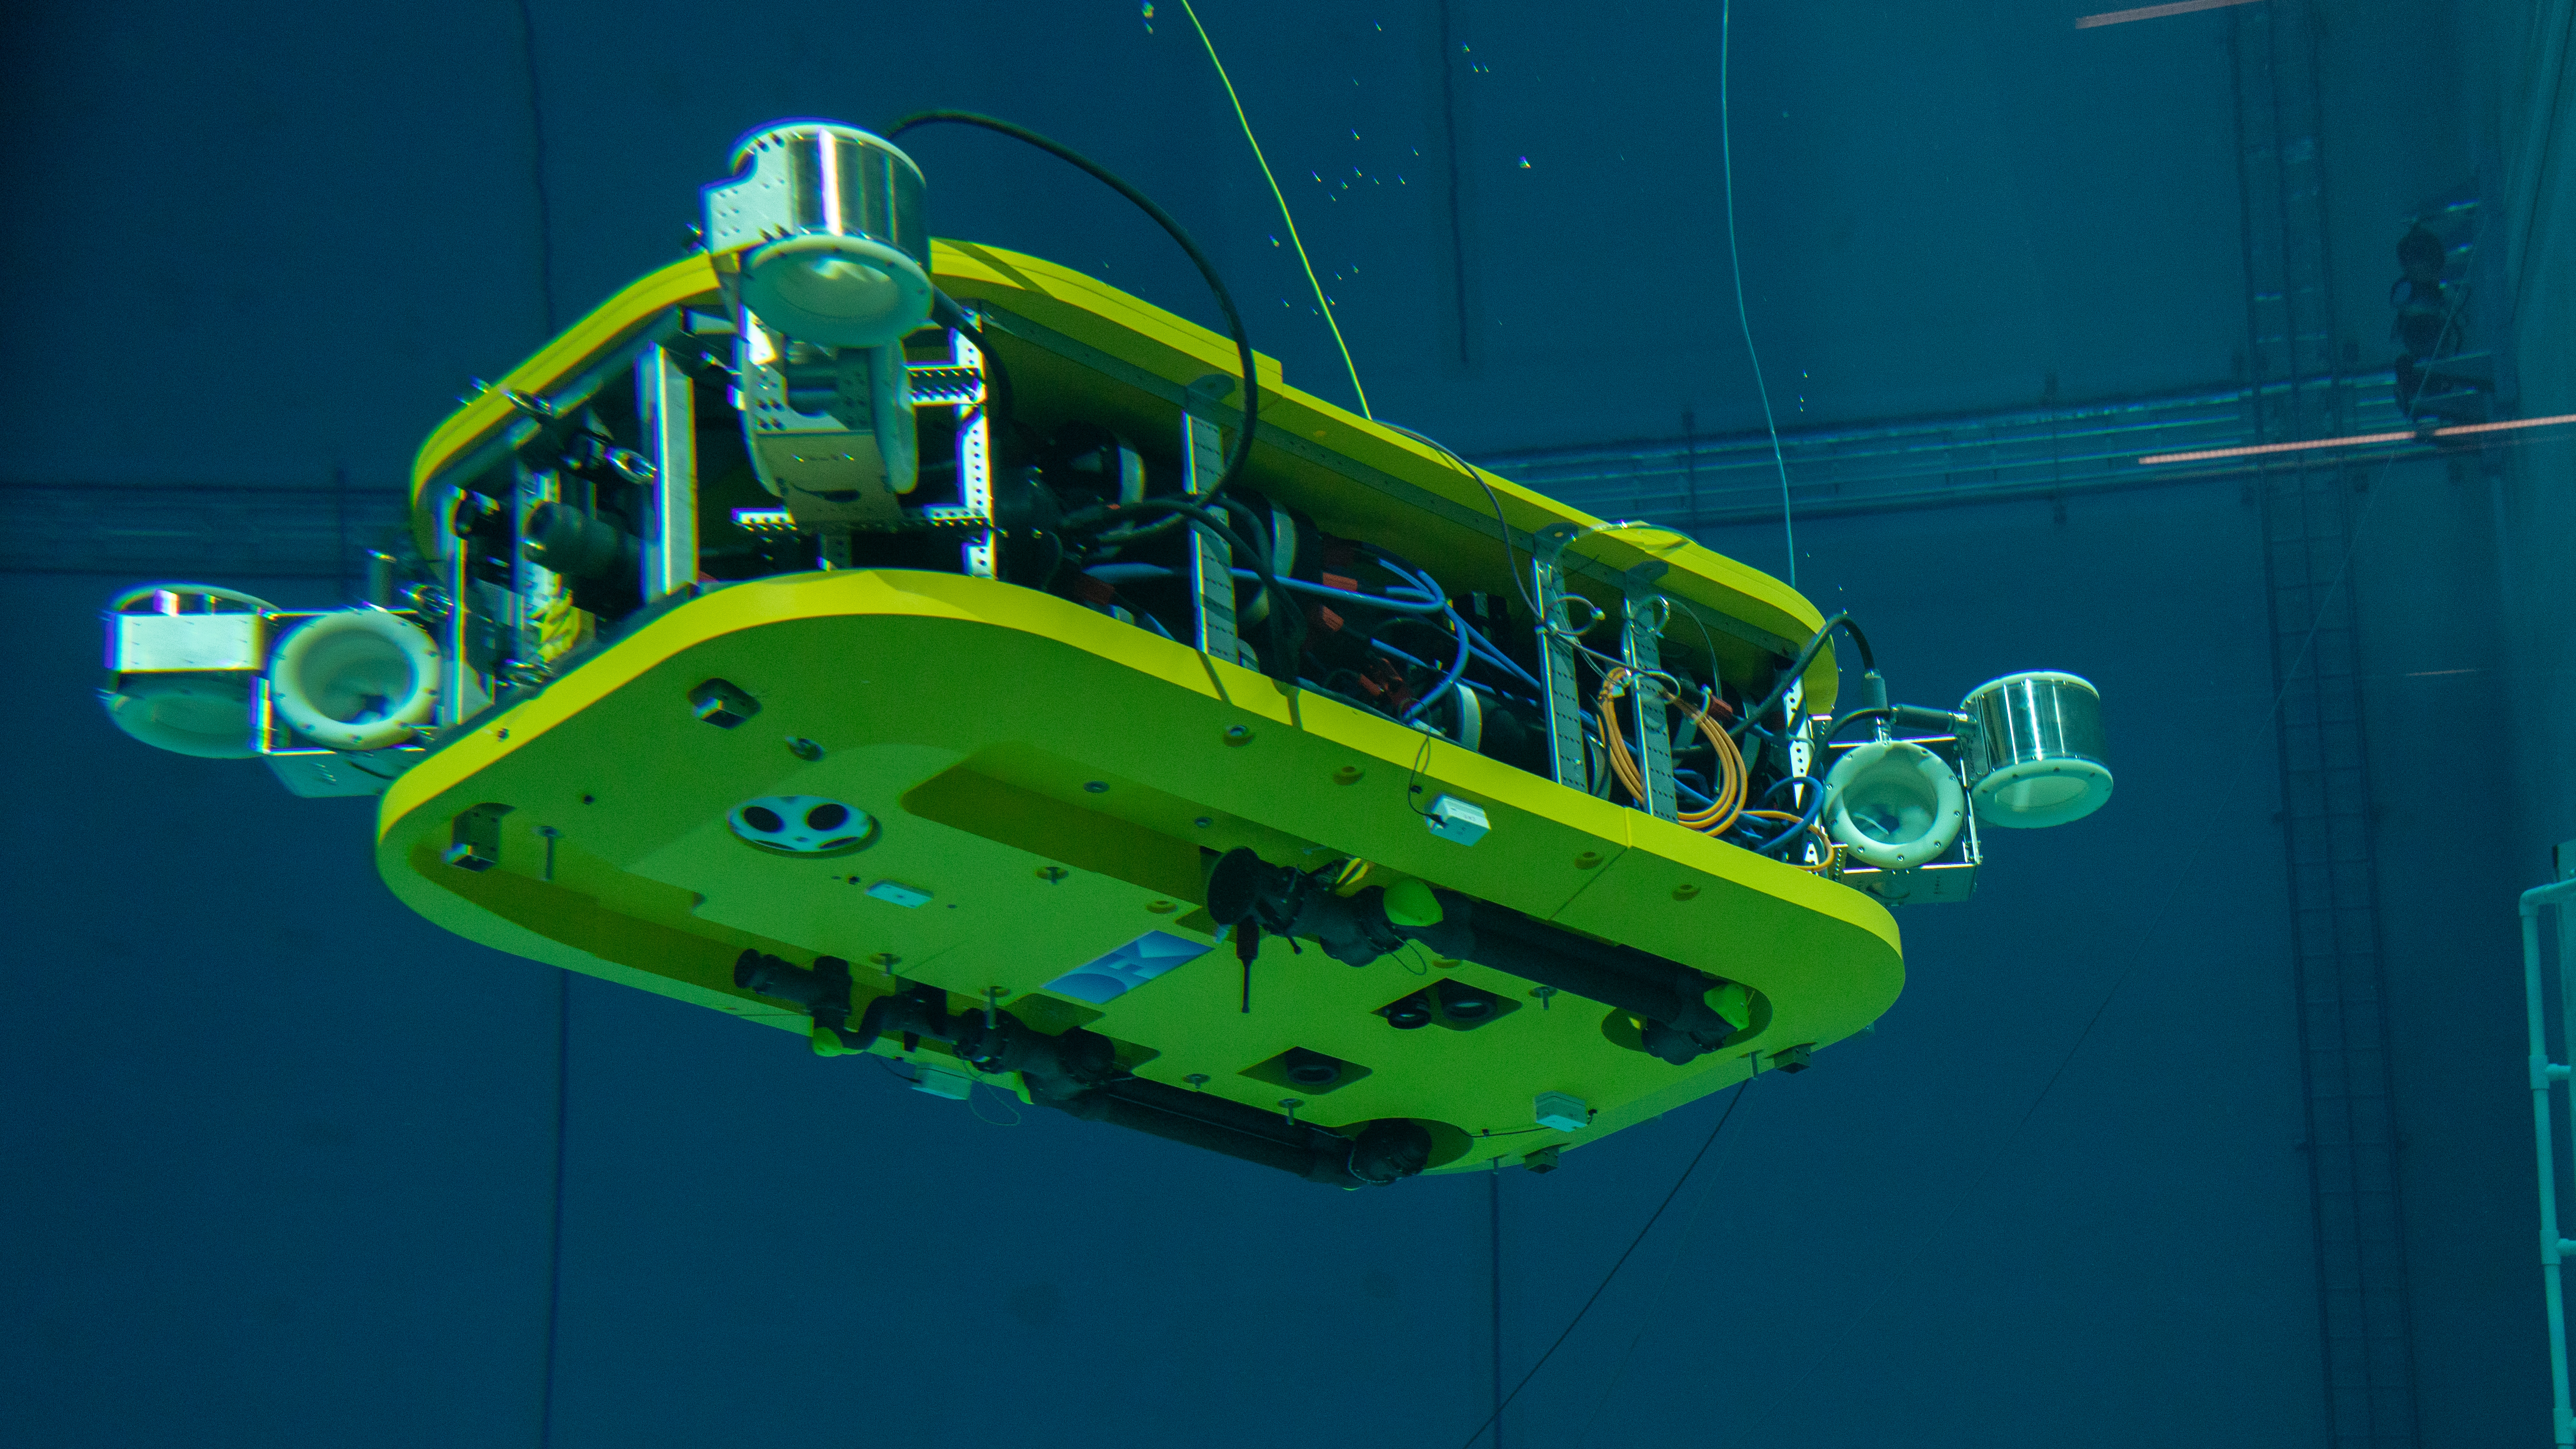
\includegraphics[width=\textwidth]{Phd_thesis/chapters/1.Introduction/figures/cuttlefish.jpg}
        \caption{DFKI Cuttlefish autonomous underwater vehicle \cite{christensen_cuttlefish_nodate}.}
        \label{fig:subfig3}
    \end{subfigure}
    \hfill
    \begin{subfigure}[b]{0.49\textwidth}
        \centering
        \includegraphics[width=\textwidth]{Phd_thesis/chapters/1.Introduction/figures/scanfish_towed.jpg}
        \caption{EIVA ScanFish Rocio remotely operated towed vehicle \cite{eiva_scanfish_nodate}.}
        \label{fig:subfig4}
    \end{subfigure}
    
    \caption{Showcase of the variety Marine Robotics Platforms.}
    \label{fig:underwater_robotics_applications}
\end{figure*}


Currently, many marine robotic tasks depend on remote control (teleoperation) or semi-autonomous functions, such as executing pre-programmed paths or simple line-following maneuvers. While effective for specific, well-defined tasks, these modes often necessitate skilled human pilots and constant supervision, limiting mission duration, complexity, and operational range.

The drive towards fully autonomous marine systems stems from the need to enhance operational safety, increase mission efficiency and capability, and reduce operational costs. By minimizing direct human intervention, autonomy mitigates the risk of human error, enables longer and more complex missions in challenging environments, and ultimately lowers operational expenses.


% --- Challenges to Autonomy ---
Achieving reliable underwater autonomy, however, requires overcoming fundamental challenges inherent to the complex and dynamic marine environment. Key among these are:

\begin{itemize}
    \item \textbf{Safe Navigation:} Ensuring safe navigation is essential, including robust obstacle avoidance and adherence to physical constraints. Many marine robots are tethered, so preventing tether entanglement during operation is a critical safety consideration.

    \item \textbf{Precise and Robust Trajectory Following:} The ability to accurately follow desired trajectories under disturbances such as ocean currents is fundamental for mission success in complex marine environments.

    \item \textbf{Generalizability Across Different Platforms:} Control and planning methods should transfer across a wide range of robotic platforms—such as UAVs, AUVs, and systems with varying sizes and degrees of freedom—without the need for substantial redesign or tuning.
\end{itemize}


















